\section*{Figures}

\begin{figure}[h]
\centering
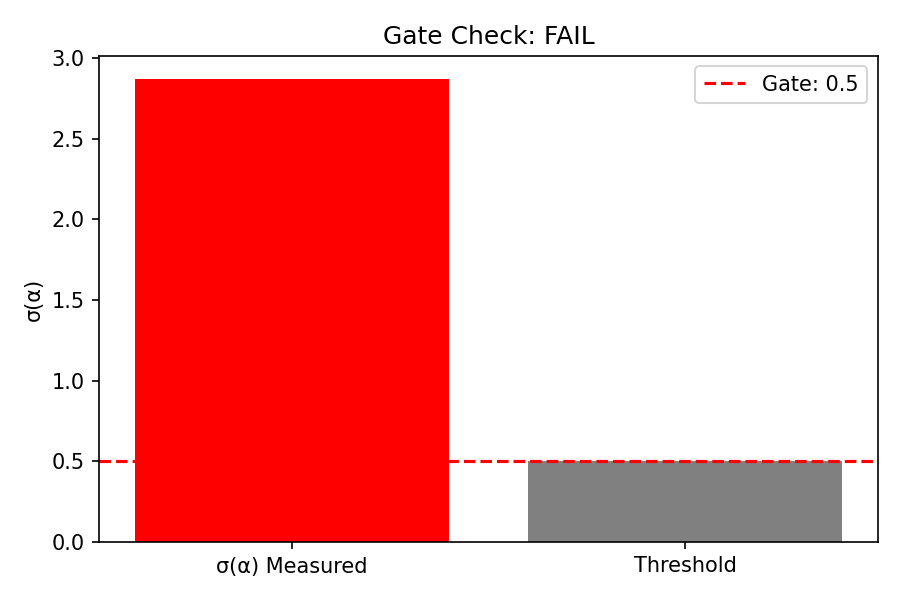
\includegraphics[width=0.8\columnwidth]{figures/gate_check.png}
\caption{Gate check visualization showing variance threshold assessment.}
\label{fig:gate}
\end{figure}

\begin{figure}[h]
\centering
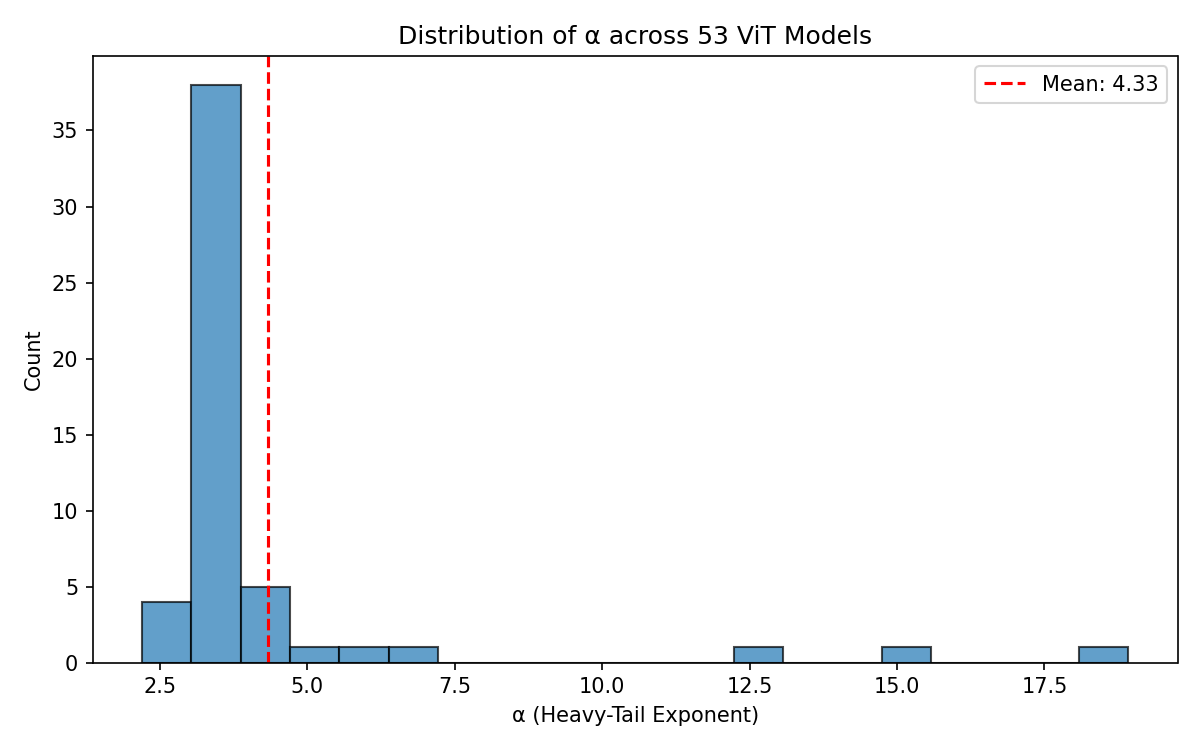
\includegraphics[width=0.8\columnwidth]{figures/alpha_histogram.png}
\caption{Distribution of $\alpha$ across 53 ViT models. The heavy right tail indicates presence of outliers from task-specific fine-tuning.}
\label{fig:histogram}
\end{figure}

\begin{figure}[h]
\centering
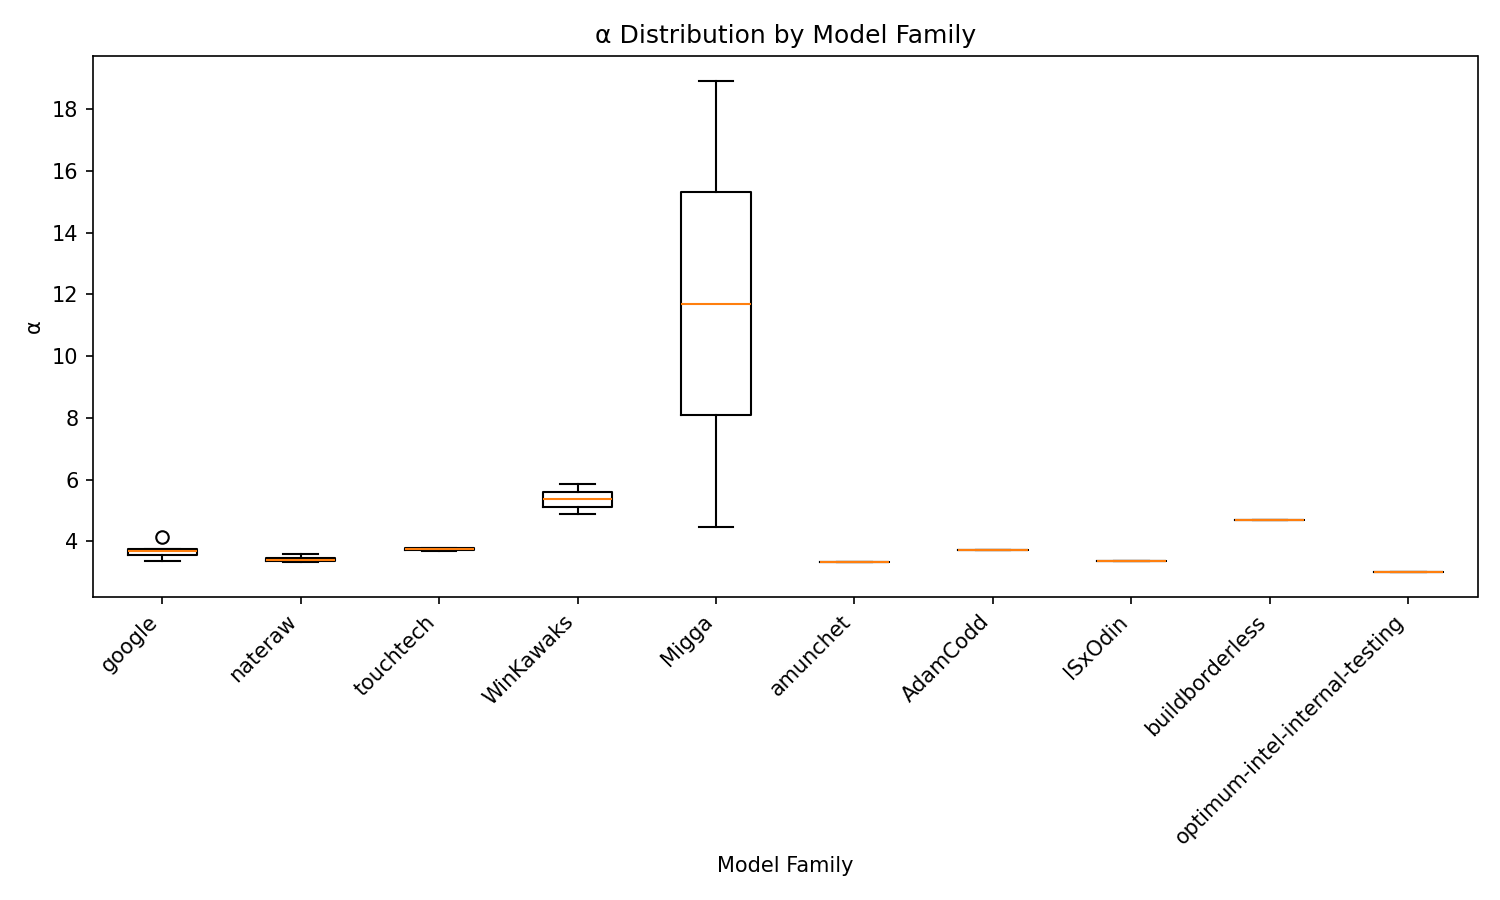
\includegraphics[width=0.8\columnwidth]{figures/family_boxplot.png}
\caption{$\alpha$ values by model family. Within-family variance (google/vit-*) is substantially lower than cross-family variance.}
\label{fig:family}
\end{figure}

\begin{figure}[h]
\centering
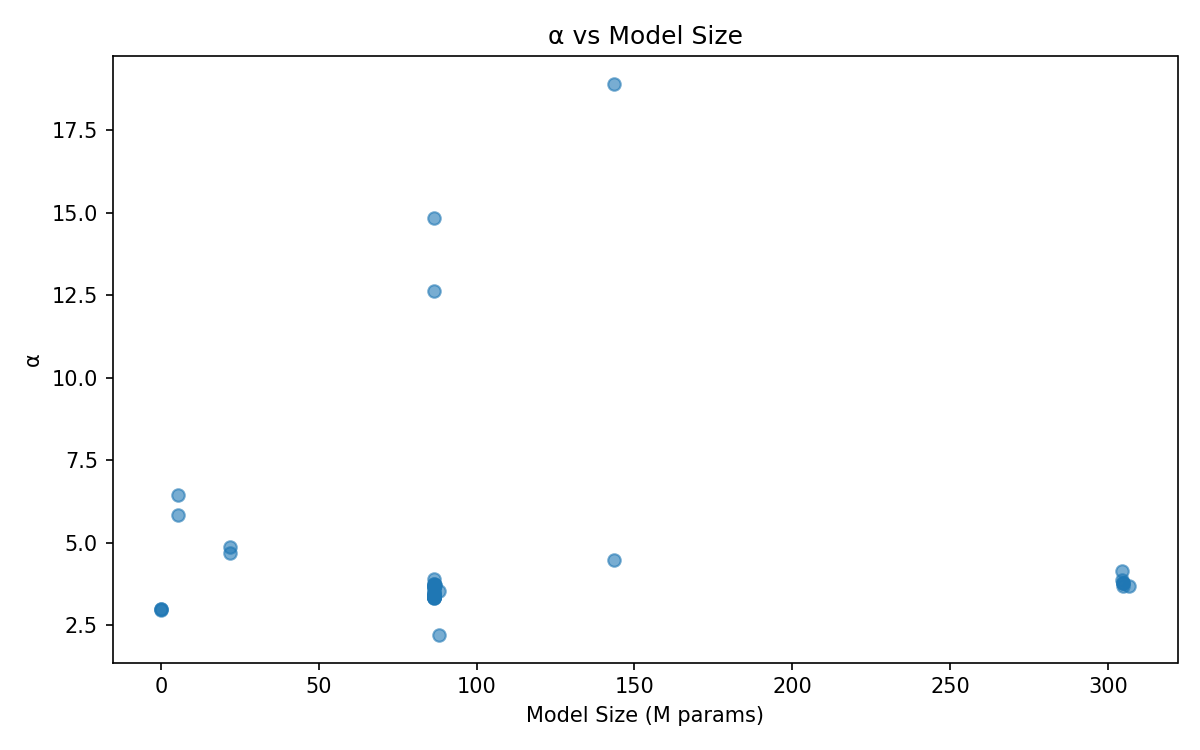
\includegraphics[width=0.8\columnwidth]{figures/alpha_vs_size.png}
\caption{$\alpha$ versus parameter count. No strong correlation observed, suggesting model size does not determine heavy-tailed behavior.}
\label{fig:size}
\end{figure}
